% =============================================================================
%  review_round5.tex -- Reviewer report, analysis of the comments, and revision
%  notes for main.tex (round 5). Compile with pdfLaTeX.
% =============================================================================
\documentclass[10pt,a4paper]{article}
\usepackage[margin=2.2cm]{geometry}
\usepackage[T1]{fontenc}
\usepackage{mathptmx}
\usepackage{amsmath,amssymb}
\usepackage{booktabs,longtable,array,tabularx}
\usepackage{graphicx}
\usepackage[font=small]{caption}
\usepackage{subcaption}
\usepackage{xcolor}
\usepackage{enumitem}
\usepackage[colorlinks=true,linkcolor=blue!50!black,urlcolor=blue!50!black]{hyperref}
\setlist{itemsep=2pt,topsep=3pt}
\graphicspath{{review_round5_figs/}}
\newcommand{\code}[1]{\texttt{#1}}
\newcommand{\yes}{\textcolor{green!45!black}{Yes}}
\newcommand{\no}{\textcolor{red!70!black}{No}}
\newcommand{\partly}{\textcolor{orange!80!black}{Partly}}

\title{Review Report and Revision Notes (Round 5)\\[3pt]
\large Two-Timescale Secure Transmission for Movable Antenna-Enabled Multiuser Systems With Statistical Eavesdropper CSI}
\author{}
\date{}

\begin{document}
\sloppy
\maketitle

\noindent This document has three parts. Part~\ref{part:review} is a reviewer report written as for an IEEE Transactions journal (TCOM/TWC) on the version of \code{main.tex} before this round (commit \code{aa01467}, 16 pages). Part~\ref{part:analysis} analyzes the validity and feasibility of every comment and documents how each one was implemented. Part~\ref{part:questions} answers the five questions raised by the author: the page count, the figure design (in particular Figs.~3 and 4), the number of FPA benchmarks, whether the old Fig.~6 is needed, and which version of Fig.~8 is better. Figure and equation numbers refer to the \emph{old} manuscript in Part~\ref{part:review} and to the \emph{revised} manuscript in Parts~\ref{part:analysis} and~\ref{part:questions} unless stated otherwise.

\tableofcontents

% =============================================================================
\part{Reviewer Report}\label{part:review}
% =============================================================================

\section{Summary of the submission}
The manuscript considers the downlink of a multiuser system in which a base station (BS) with $N$ movable antennas (MAs) serves $M$ single-antenna legitimate users (LUs) in the presence of a single-antenna passive eavesdropper (Eve) whose statistical CSI (Rician factor, large-scale fading, and angle of departure, AoD) is known. A two-timescale design is proposed: the antenna positions and a long-term power allocation (per-user powers $p_m$ and the AN power $q$ per null-space dimension) are optimized from statistical CSI once per frame, whereas zero-forcing (ZF) precoding and isotropic null-space AN are computed from the instantaneous CSI of the LUs in each coherence interval. The authors
(i) prove that the information leakage and the AN received by Eve are conditionally independent given the LU channels (Lemma~2);
(ii) approximate the average LoS energies of Eve along the ZF direction and in the null space by replacing $(\mathbf F^H\mathbf F)^{-1}$ with the inverse of its mean and calibrating the NLoS share by the trace identity (Lemma~3), which yields a closed-form ergodic wiretap rate (Proposition~1) and an approximate ESSR that depends on the positions only through three geometric quantities;
(iii) solve the ESSR maximization by alternating optimization (AO), with a secrecy water-filling power allocation (Proposition~3) and element-wise MM position updates with analytical gradients; and
(iv) compare the design with a rate-oriented two-timescale MA design, antenna selection (AS), and two fixed-position arrays (FPAs).

\section{Overall assessment and recommendation}
The topic is timely: MA-aided physical layer security is an active area, and the two-timescale setting is well motivated for a passive Eve whose instantaneous CSI is unavailable. I checked the main derivations and found them correct: Lemma~1 coincides with~[16, Sec.~IV-A]; the conditional independence in Lemma~2 follows from the orthonormality of $[\bar{\mathbf w}_m,\mathbf U]$; both special cases of Lemma~3 ($\bar{\mathbf F}=\mathbf 0$ exact; $\bar{\mathbf F}=\varrho\bar{\mathbf F}_0$, $\varrho\to\infty$, asymptotically exact) hold; the single-LU expressions in Remark~3 and the high-SNR splitting $\alpha^\star=1/(1+\sqrt\Theta)$ in Remark~4 are correct; and the secrecy water-filling solution in Proposition~3 is the positive root of the KKT quadratic written in a stable form. The benchmarks are generally fair (the same power allocation for all position designs, shared AoD realizations, and exact Monte Carlo evaluation), and the simulation code is available. The observation that the MAs improve secrecy even for a single LU, unlike the rate-oriented design, and reduce the AN power is a genuine contribution.

My main concerns are (a) the length and focus of the manuscript, (b) the presentation quality of several figures, (c) the absence of a robustness check for the most critical modeling assumption, i.e., the statistical CSI of Eve, and (d) the strength of the AS benchmark. All of them can be addressed within one revision.

\noindent\textbf{Recommendation:} Major revision.

\section{Major comments}
\begin{description}[leftmargin=0pt]
\item[M1 (Length and focus).] At 16 pages, the manuscript exceeds the typical length of a regular paper, and the main messages are diluted.
\begin{enumerate}[label=\alph*)]
\item Fig.~6(a) (ESSR vs.\ the angular offset $\Delta$) and Fig.~7 (ESSR vs.\ the region size $A$) convey the same physics: the gain is governed by whether the region can resolve the angular separation between Eve and LU~1 (resolution of the order of $\lambda/A$). Two sentences with numbers suffice for $\Delta$.
\item Fig.~6(b) confirms Remark~3, which is already proven analytically; a few numbers (secrecy rate and AN fraction at one $\Delta$) suffice.
\item The two FPA benchmarks are redundant for $M=3$: the sparse FPA never outperforms the rate-oriented MA by more than 0.8\% in Figs.~5--7 (at 20~dB, 17.75 vs.\ 17.87~bps/Hz), and the conclusion it supports (the gain is not merely due to a larger aperture) is already established by the rate-oriented MA, which uses the same region. Keep the conventional $\lambda/2$ FPA, which is the standard reference in the MA literature, and mention the sparse array in one sentence.
\item Fig.~8 uses two stacked panels for the ablation of a secondary component (see M6).
\item Table~I (key symbols) is not essential, and several passages repeat earlier material: the protocol motivation in Section~II-B repeats the Introduction, the paragraph on the properties of the ZF-AN design is long, the discussion after Lemma~2 can be shortened, and the displayed array correlations in Remark~2 can be inlined.
\end{enumerate}
Please condense the manuscript to about 13 pages.

\item[M2 (Figure quality).] Several figures fall short of the presentation standard of IEEE Transactions.
\begin{enumerate}[label=\alph*)]
\item Fig.~3: the ergodic wiretap sum rate, which validates the main analytical result (Proposition~1), is compressed into the bottom tenth of a 0--45~bps/Hz axis shared with the LU rates, so that its accuracy cannot be judged. The factorized legend uses a black circle for ``Monte Carlo'' while the compact FPA also uses circles, and the markers of the two configurations overlap. Please plot the LU and Eve rates on separate $y$-scales (e.g., two stacked axes per panel) and use the convention ``lines: analysis, markers: simulation'' stated in the caption.
\item Fig.~4: three stacked panels with boxed SNR labels, a full-width legend frame, and staggered markers make a simple convergence result look cluttered and occupy 3~in of column height. One panel at the default SNR is sufficient; the other SNRs can be summarized in the text.
\item General: heavy lines (1.2~pt) and large markers; legends that touch the data (Fig.~5(b)) or occupy the upper third of the axes (Figs.~5(b), 6, and~7); red--green color pairs, which are not distinguishable for color-blind readers; non-integer font sizes; inconsistent legend placement and axis ranges; and raster graphics. Please use one style per scheme across all figures, 8--9~pt fonts matching the text, colors that remain distinguishable in grayscale through line styles and markers, and vector graphics for the final version.
\end{enumerate}

\item[M3 (Robustness to imperfect statistical CSI of Eve).] The design explicitly decorrelates the LoS component of Eve from those of the LUs (Remark~2), so its benefit hinges on the accuracy of the AoD of Eve, which in practice is obtained by sensing or localization [15]. The manuscript defers this to future work. A basic sensitivity study is necessary to judge the practicality: design with an AoD of Eve perturbed by $\varepsilon$ in a random direction, evaluate with the true AoD, and report the ESSR of all schemes for a few values of $\varepsilon$, including one comparable to $\Delta$.

\item[M4 (Strength of the AS benchmark).] The AS candidates form a compact $\lambda/2$-spaced $4\times4$ array (aperture $1.5\lambda$), whereas the MAs move within $4\lambda\times4\lambda$. The statement that ``AS cannot exploit a larger region'' is therefore an artifact of the candidate layout. Please evaluate an AS benchmark whose $2N$ candidates span the movable region, and qualify the claims in the abstract, the contributions, and Section~V accordingly.

\item[M5 (Impact of the conservative LU-rate approximation).] Lemma~1 underestimates the LU rates by about 1.5--1.7~bps/Hz, i.e., by about 9\% of the ESSR at 20~dB. The argument that this gap barely depends on the antenna positions is supported by only two configurations (compact FPA and random MA). Please provide evidence at the optimized designs, e.g., the gap between the Monte Carlo and the approximate ESSR for every scheme, and the agreement between the predicted and the actual relative gains.

\item[M6 (Design of the power-allocation figure).] The current Fig.~8 (ESSR vs.\ the fading spread $\varsigma$ at 0 and 10~dB, two stacked panels) is dominated by a trend that is unrelated to the power allocation: all ESSRs decrease because LUs~2 and~3 lose channel gain. The gain of the per-user allocation must be read off from small gaps between nearly parallel curves (at 10~dB, the proposed and the optimized-$\alpha$ curves overlap for $\varsigma\le10$~dB), and the vanishing gain at high SNR, a key message, is only stated in the text. A single panel with the relative ESSR loss of the equal-power benchmarks versus the SNR, for identical and heterogeneous LUs, would convey all three conclusions (the information--AN splitting is dominant; per-user allocation matters for heterogeneous LUs at low-to-moderate SNR; the gain vanishes at high SNR) in a quarter of the space.
\end{description}

\section{Minor comments}
\begin{enumerate}[label=m\arabic*.,leftmargin=*]
\item The abstract (about 330 words) exceeds the 150--250 words recommended by IEEE.
\item The 16.6\% gain over AS in the abstract and the contributions should state the AS configuration (see M4).
\item ``Algorithm~2 is guaranteed to converge'' should read ``the objective value of Algorithm~2 is guaranteed to converge''; the convergence of the iterates to a stationary point is not shown.
\item References must be numbered in the order of first citation; [26] (Sun \emph{et al.}) is cited before [25] (Beck).
\item Section~V-C: report the convergence statistics for the setting shown in the figure; if a single panel is used, give the other SNRs in one sentence.
\item Table~II: state that the design without AN is obtained by Algorithm~2 with $q=0$.
\item Notation: several standard definitions ($\mathbb C^{a\times b}$, $\nabla$, $\mathcal O(\cdot)$, $\triangleq$) can be removed.
\item Fig.~5(b): the $y$-label repeats the caption; ``AN power fraction'' suffices.
\item Section~V-G quotes the 20~dB power-allocation results only in the text; see M6.
\item Update the arXiv references [14] and [15] if published versions appear before submission.
\end{enumerate}

\section{Optional comments}
\begin{enumerate}[label=O\arabic*.,leftmargin=*]
\item An instantaneous-CSI (single-timescale) MA design would quantify the price of the two-timescale operation. I understand that it requires the CSI over the entire region and a different algorithm; a remark would suffice.
\item Multiple or multi-antenna eavesdroppers and imperfect CSI of the LUs are natural extensions; the conclusion mentions them.
\end{enumerate}

% =============================================================================
\part{Analysis of the Comments and Implemented Revisions}\label{part:analysis}
% =============================================================================

\section{Validity and feasibility}
Table~\ref{tab:triage} classifies every comment. ``Valid'' means that the comment identifies a real weakness; ``feasible'' means that it can be addressed within this revision without new theory and within the page budget. Every valid and feasible comment was implemented.

{\small
\begin{longtable}{p{1.3cm}p{0.9cm}p{1.3cm}p{11.2cm}}
\caption{Triage of the reviewer comments}\label{tab:triage}\\
\toprule
Comment & Valid & Feasible & Action \\ \midrule
\endfirsthead
\toprule
Comment & Valid & Feasible & Action \\ \midrule
\endhead
M1 & \yes & \yes & Old Fig.~6 removed (key numbers in Section~V-E), sparse FPA removed from all figures (one sentence in Section~V-A), Fig.~8 reduced to one panel (new Fig.~7), Fig.~4 reduced to one panel, Table~I (key symbols) removed, prose condensed throughout. \textbf{16 $\to$ 13 pages}; source words $12{,}338\to9{,}885$. \\
M2 & \yes & \yes & New common figure style (\code{fig\_style.m}, \code{scheme\_style.m}); Fig.~3 with stacked LU/Eve axes; Fig.~4 single panel; color-blind-safe palette; legends in free regions; integer font sizes; fixed margins. Vector PDFs are exported by MATLAB; Octave (used here) exports 600-dpi PNGs, see Section~\ref{sec:q2}. \\
M3 & \yes & \yes & New simulation \code{extra\_eve\_aod\_error.m}; new paragraph in Section~V-D. Losses of the proposed design: 0.2\%, 0.3\%, 2.2\%, and 8.3\% for $\varepsilon=0.01$, 0.02, 0.05, and 0.1~rad; it remains the best scheme for all $\varepsilon$. \\
M4 & \yes & \yes & New simulation \code{extra\_as\_region.m} (AS with $2N$ candidates spanning $\mathcal C$); new sentences in Section~V-E; claims in the abstract and contributions qualified. The proposed design is better by 3.7\%--4.3\% for $A\ge3\lambda$ (Section~\ref{sec:m4}). \\
M5 & \yes & \yes & Evidence from the existing data added to Section~V-B: the approximation gap is 1.52--1.73~bps/Hz for all schemes at the optimized designs, and the predicted relative gains deviate from the Monte Carlo ones by at most 2.2 percentage points. \\
M6 & \yes & \yes & Restored the round-2 design (single panel, relative ESSR loss vs.\ SNR), restyled; no new simulation needed (Section~\ref{sec:q5}). The fading-spread sweep is summarized in one sentence. \\
m1 & \yes & \yes & Abstract shortened to 248 words. \\
m2 & \yes & \yes & Abstract: ``outperforms antenna selection with twice as many antennas''; contributions report both AS variants (16.6\% and 3.9\%). \\
m3 & \yes & \yes & Reworded in Section~IV-D. \\
m4 & \yes & \yes & Bibliography reordered (also Horn/Ngo, whose order changed after condensing); the order of first citation is now verified automatically. \\
m5 & \yes & \yes & Section~V-C reports the 20~dB statistics (shown) and summarizes 10/30~dB. \\
m6 & \yes & \yes & Section~V-A: ``i.e., Algorithm~2 with $q=0$''. \\
m7 & \yes & \yes & Notation paragraph condensed. \\
m8 & \yes & \yes & $y$-label changed. \\
m9 & \yes & \yes & Covered by M6. \\
m10 & \yes & -- & Left to the authors (requires checking the publication status before submission). \\
O1 & \partly & \no & A single-timescale MA design needs the CSI over the whole region in every CI and a different algorithm; it is outside the scope argued in Section~I and would add length. Not implemented. \\
O2 & \yes & \no & Requires new analysis; remains future work in Section~VI. \\
\bottomrule
\end{longtable}
}

\section{Details of the new results}
\subsection{M3: robustness to errors in the AoD of Eve}\label{sec:m3}
All schemes are designed with an AoD of Eve deviating from the true one by $\varepsilon$ in a random direction (\code{design\_scenario.m}; the same direction is used for all $\varepsilon$) and evaluated by Monte Carlo simulation with the true AoD ($20$~dB, 100 AoD realizations). For $\varepsilon=0$, the results coincide with the $20$~dB point of Fig.~5 to all digits, which verifies the new code path.

\begin{center}\small
\begin{tabular}{lccccc}
\toprule
$\varepsilon$ (rad) & 0 & 0.01 & 0.02 & 0.05 & 0.1 \\ \midrule
Proposed & 20.10 & 20.06 & 20.03 & 19.65 & 18.43 \\
Rate-oriented MA & 17.87 & 17.86 & 17.86 & 17.83 & 17.75 \\
AS & 17.24 & 17.24 & 17.22 & 17.16 & 16.97 \\
FPA & 15.82 & 15.82 & 15.81 & 15.81 & 15.80 \\ \midrule
Gain over rate-oriented MA & 12.5\% & 12.3\% & 12.1\% & 10.2\% & 3.8\% \\
Realizations with proposed $>$ rate-oriented & 100\% & 100\% & 100\% & 98\% & 76\% \\
\bottomrule
\end{tabular}
\end{center}
The benchmarks are almost unaffected, since their positions do not depend on Eve (only their power allocation and, for AS, the selection do). The proposed design degrades gracefully: even when the error equals the angular offset between Eve and LU~1 ($\varepsilon=\Delta=0.1$~rad), it remains the best scheme on average.

\subsection{M4: AS with candidates spanning the movable region}\label{sec:m4}
\begin{center}\small
\begin{tabular}{lcccccc}
\toprule
$A/\lambda$ & 1.5 & 2 & 3 & 4 & 5 & 6 \\ \midrule
Proposed & 17.21 & 18.05 & 19.28 & 20.10 & 20.69 & 21.05 \\
AS, candidates span $\mathcal C$ & 17.24 & 17.66 & 18.48 & 19.34 & 19.95 & 20.26 \\
AS, compact $\lambda/2$ candidates (Fig.~6) & 17.24 & 17.24 & 17.24 & 17.24 & 17.24 & 17.24 \\
Gain of proposed over region-wide AS & $-0.2\%$ & 2.2\% & 4.3\% & 3.9\% & 3.7\% & 3.9\% \\
\bottomrule
\end{tabular}
\end{center}
This is an honest and important qualification. When its 16 candidates span the region (spacing $A/3$), AS also exploits the enlarged aperture and, since it uses the same Eve-aware metric (Proposition~1), recovers most of the gain: at $A=4\lambda$, it achieves 19.34~bps/Hz, i.e., the proposed design is better by 3.9\% (in 81 of the 100 AoD realizations) instead of 16.6\%. For $A=1.5\lambda$, the candidate grid coincides with the compact one, and the two AS variants coincide, which is a consistency check. Two conclusions follow, and both are now stated in the manuscript: (i) the dominant source of the secrecy gain is the \emph{Eve-aware} geometry enabled by Proposition~1, which benefits both MA and AS arrays; (ii) the MA design achieves it with half the number of antennas and without an RF switching network spanning the region, and still outperforms the region-wide AS. The compact AS remains in the figures because it is the common AS configuration; if a reviewer asks for it, the region-wide AS can be added as a fifth curve to Fig.~6 with \code{extra\_as\_region.mat}.

\subsection{M5: the approximation at the optimized designs}\label{sec:m5}
From the existing Fig.~5 data at $20$~dB (no new simulation):
\begin{center}\small
\begin{tabular}{lccccc}
\toprule
 & Proposed & Rate-oriented MA & AS & FPA & Sparse FPA \\ \midrule
Monte Carlo ESSR (bps/Hz) & 20.10 & 17.87 & 17.24 & 15.82 & 17.75 \\
Approximate ESSR (27) & 18.37 & 16.33 & 15.71 & 14.21 & 16.16 \\
Gap & 1.73 & 1.53 & 1.52 & 1.61 & 1.59 \\
Gain of proposed, Monte Carlo & -- & 12.5\% & 16.6\% & 27.1\% & 13.2\% \\
Gain of proposed, predicted by (27) & -- & 12.5\% & 16.9\% & 29.2\% & 13.7\% \\
\bottomrule
\end{tabular}
\end{center}
The gap is nearly scheme-independent, and the predicted relative gains deviate from the true ones by at most 2.2 percentage points. Hence, the conservative approximation preserves the ranking of the designs, which is what the optimization requires. One sentence with these numbers was added to Section~V-B.

% =============================================================================
\part{Answers to the Author's Questions}\label{part:questions}
% =============================================================================

\section{Is 16 pages too long? What was streamlined?}\label{sec:q1}
Yes. For a regular paper in IEEE TCOM/TWC, about 12--13 pages in the two-column format is typical, and every page beyond that must be justified by content. The revised manuscript has \textbf{13 pages} (abstract 248 words; source text 9,885 words instead of 12,338), although two robustness checks were added. The cuts were made where they cost the least information:
\begin{itemize}
\item \textbf{Simulation design.} The old Fig.~6 (angular offset; single LU, a \texttt{figure*}) was removed and replaced by four sentences with the key numbers. The sparse FPA was removed from all figures. The power-allocation figure went from two stacked panels to one, and the convergence figure from three stacked panels to one.
\item \textbf{Analysis sections.} Table~I (key symbols) was removed; the motivation of the protocol (repeating the Introduction), the properties of the ZF-AN design, the discussion after Lemma~2, Remark~2 (array correlations inlined), the complexity paragraph, and the conclusion were condensed. No equation, lemma, proposition, proof, or appendix was removed, and all derivations are unchanged.
\item \textbf{Introduction.} The challenges paragraph and the literature review were tightened; the four contributions were kept.
\end{itemize}
Further cuts would remove content that reviewers expect (e.g., Algorithm~1, the protocol figure, or Appendix~B with the gradients needed for reproducibility); I do not recommend them.

\section{Figure design (in particular Figs.~3 and 4)}\label{sec:q2}
All figures were redrawn with one common style, defined in \code{fig\_style.m} and \code{scheme\_style.m}:
\begin{itemize}
\item one IEEE column per panel ($3.5\times2.45$~in) with fixed margins, included at \verb|\columnwidth| or \verb|0.48\textwidth|, so that the fonts appear at their nominal size: 8-pt ticks, 9-pt labels, and 7-pt legends in Times, matching the IEEEtran body text; all font sizes are integers;
\item a color-blind-safe palette that is also distinguishable in grayscale through line styles and markers: proposed (red, solid, circles), rate-oriented MA (blue, solid, squares), AS (orange, dash-dotted, triangles), FPA (dark gray, dashed, diamonds); hollow markers and 1.0-pt lines instead of 1.2-pt lines;
\item a light solid grid, axes drawn above the curves, and compact legends with thin frames placed in empty regions; no legend touches a curve (in the old Fig.~5(b), the FPA markers touched the legend), and the axis ranges no longer reserve a third of the plot for the legend.
\end{itemize}

\paragraph{Fig.~3 (accuracy).} The old figure plotted the LU and Eve rates on one 0--45~bps/Hz axis (Fig.~\ref{fig:cmp3}, top). The Eve rates, which validate Proposition~1, the new result of the paper, were squeezed into the bottom tenth of the axis, so that the agreement could not be seen; the legend mixed a configuration key with a ``Monte Carlo'' key that reused the circle marker of the FPA. The new figure uses two stacked axes per panel with a common $x$-axis: the LU rates on top and the Eve rates at the bottom, each on its own scale. The 0.16~bps/Hz accuracy of Proposition~1 and the conservative gap of Lemma~1 are now visible. The legend has two entries (FPA, random MA), and the caption states ``lines: closed-form approximations; markers: Monte Carlo simulations'', which is the usual IEEE convention.

\paragraph{Fig.~4 (convergence).} The old figure had three stacked panels (30/20/10~dB) with boxed SNR labels and a full-width legend frame (Fig.~\ref{fig:cmp4}, left). The new figure shows one panel at the default SNR of 20~dB with the three initializations, and the text reports the statistics for 10 and 30~dB (95\% of the improvement within 25--57 iterations; the UPA initialization is always best). The figure is now a standard single-column convergence plot.

\begin{figure}[p]
\centering
\begin{subfigure}{0.46\textwidth}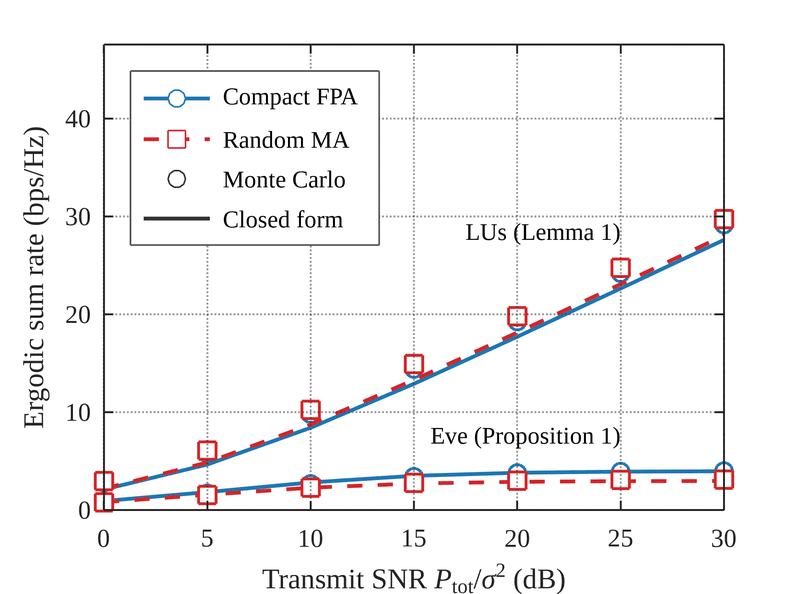
\includegraphics[width=\linewidth]{old_fig3a}\caption{Old Fig.~3(a)}\end{subfigure}\hfill
\begin{subfigure}{0.46\textwidth}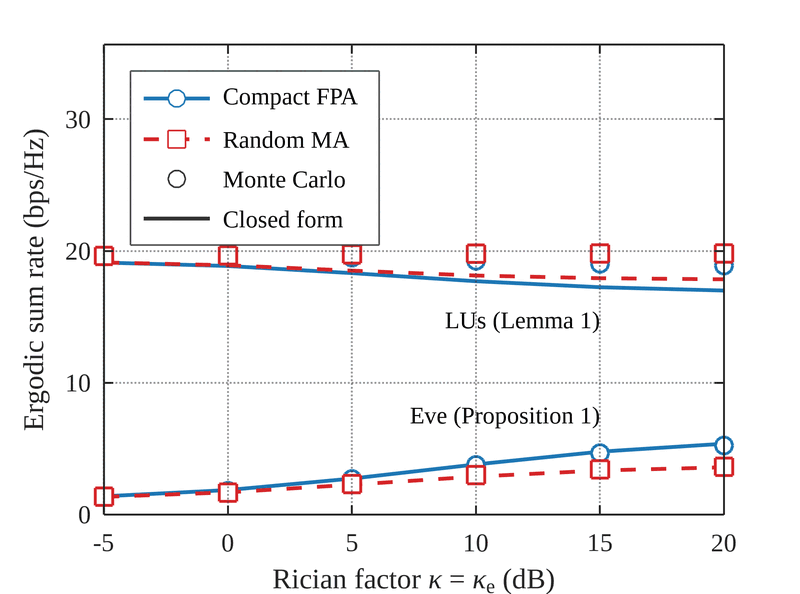
\includegraphics[width=\linewidth]{old_fig3b}\caption{Old Fig.~3(b)}\end{subfigure}\\[4pt]
\begin{subfigure}{0.46\textwidth}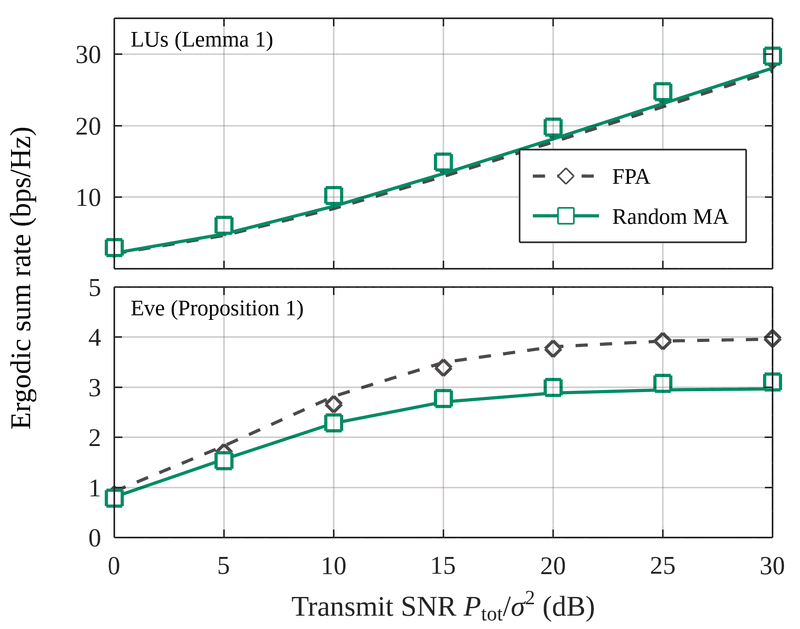
\includegraphics[width=\linewidth]{new_fig3a_accuracy_snr}\caption{New Fig.~3(a)}\end{subfigure}\hfill
\begin{subfigure}{0.46\textwidth}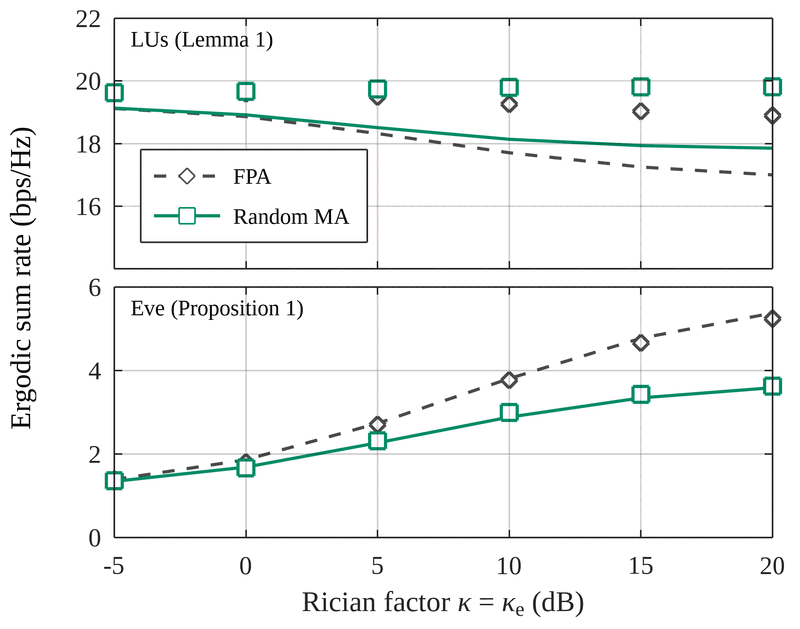
\includegraphics[width=\linewidth]{new_fig3b_accuracy_kappa}\caption{New Fig.~3(b)}\end{subfigure}
\caption{Fig.~3 before and after. In the new version, the Eve rates (Proposition~1) have their own axis.}
\label{fig:cmp3}
\end{figure}

\begin{figure}[p]
\centering
\begin{subfigure}{0.46\textwidth}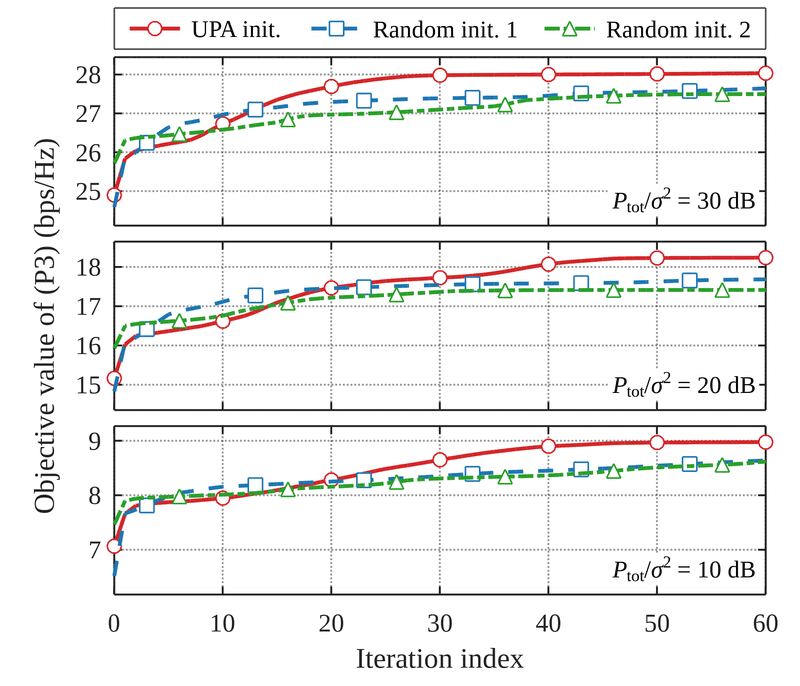
\includegraphics[width=\linewidth]{old_fig4}\caption{Old Fig.~4}\end{subfigure}\hfill
\begin{subfigure}{0.46\textwidth}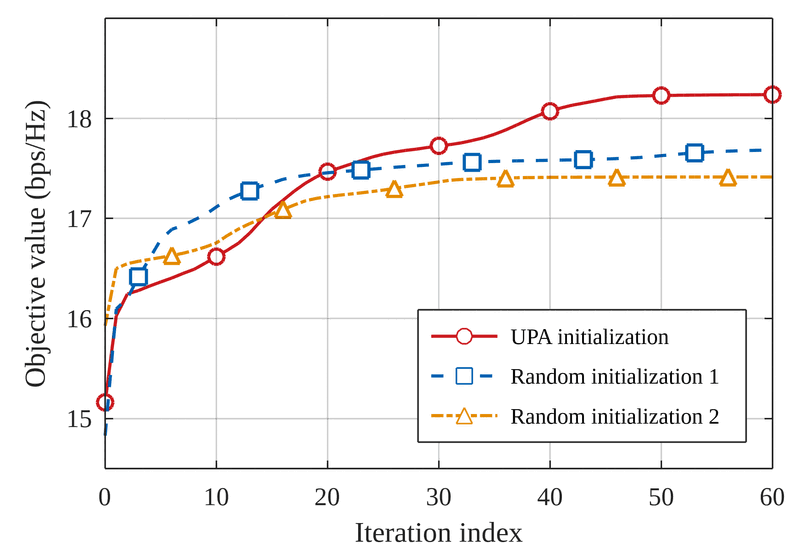
\includegraphics[width=\linewidth]{new_fig4_convergence}\caption{New Fig.~4}\end{subfigure}
\caption{Fig.~4 before and after.}
\label{fig:cmp4}
\end{figure}

\paragraph{Vector graphics.} The previous rounds and this round compute the figures with Octave, whose vector export lays out the text on a 96-dpi pixel grid: word spaces shrink or disappear (e.g., ``Ergodic sumrate'' in rotated labels), and the legend keys do not scale. Therefore, Octave exports 600-dpi PNGs, which satisfy the IEEE requirement for line art, and the manuscript uses them. In MATLAB, \code{replot\_all} exports vector PDFs with embedded fonts, which \code{main.tex} picks up automatically (\verb|\includegraphics| without extension prefers \code{.pdf}). For the final submission, please run \code{replot\_all} once in MATLAB.

\section{Too many FPA benchmarks? Keep only one?}\label{sec:q3}
Yes, one FPA is enough, and it should be the compact $\lambda/2$ array (now called ``FPA''). Reasons:
\begin{enumerate}
\item \textbf{The sparse FPA is redundant with the rate-oriented MA.} Its only purpose was to show that the gain is not merely due to a larger aperture. The rate-oriented MA already shows this, since it uses the same $4\lambda\times4\lambda$ region, and for $M=3$ it is never worse than the sparse FPA by more than 0.8\% (17.87 vs.\ 17.75~bps/Hz at 20~dB; the sparse FPA is 11\%--16\% worse at 0--5~dB). The proposed design beats both by 12.5\%--13.3\% at 20~dB. The only exception is the single-LU case, where the rate-oriented MA degenerates to the compact FPA and the sparse FPA is the strongest fixed array; its value is therefore reported in the single-LU sentence of Section~V-E (6.45 vs.\ 7.46~bps/Hz for the proposed design).
\item \textbf{The compact FPA is the standard reference.} The MA literature (including [16] and [17]) compares with the conventional $\lambda/2$ array; it is also the initialization of Algorithm~2 and the sub-array of the AS candidates.
\item \textbf{Fewer curves.} Figs.~5 and 6 now have four curves, each representing one design principle: Eve-aware MA, Eve-unaware MA, antenna selection, and a conventional array.
\end{enumerate}
To preempt the aperture question, Section~V-A keeps one sentence with the sparse-FPA numbers, and the code still evaluates it (\code{SPA\_full}).

\section{Is the old Fig.~6 redundant? Can it be removed?}\label{sec:q4}
Yes, it was removed. Its content was not wrong, but it did not justify a \texttt{figure*} (one third of a page):
\begin{itemize}
\item \textbf{Fig.~6(a) (ESSR vs.\ $\Delta$, $M=3$)} illustrates the same mechanism as the region-size figure (new Fig.~6): the gain depends on whether the aperture resolves the angular separation between Eve and LU~1. Its message fits in two sentences: the gain over the rate-oriented MA is only 0.9\% at $\Delta=0.02$~rad, peaks at 14.4\% at $\Delta=0.2$~rad, and decreases to 10.9\% at $\Delta=0.5$~rad.
\item \textbf{Fig.~6(b) (single LU)} confirms Remark~3, which is proven analytically. The decisive numbers are now in the text: at $\Delta=0.1$~rad, the secrecy rate increases from 4.22 to 7.46~bps/Hz (76.6\%), the rate-oriented MA coincides with the FPA, AS achieves 4.74~bps/Hz, and the AN fraction drops from 0.84 to 0.51.
\end{itemize}
The simulations are kept as \code{extra\_angle\_offset.m} and \code{extra\_single\_user.m}, so every quoted number remains reproducible.

\section{Fig.~8: latest or original version, and which is better?}\label{sec:q5}
\paragraph{Which version was in the manuscript.} The Fig.~8 in the manuscript before this round was the \textbf{latest (round-3) version}: ESSR versus the fading spread $\varsigma$ of the LUs, two stacked panels at 0 and 10~dB, three power allocations each (Fig.~\ref{fig:cmp8}(c), (d)). It was produced in round 3 in response to the remark that Fig.~8 did not look good; in round 4, that remark was clarified to concern Fig.~4, which was then redrawn, but the round-3 Fig.~8 was kept. In other words, the earlier design was replaced because of a misunderstanding, not because it was worse. Two earlier versions exist in the git history:
\begin{itemize}
\item \textbf{Round 1} (commit \code{406d979}, Fig.~\ref{fig:cmp8}(a)): ``ESSR gain over equal power (\%)'' vs.\ $\varsigma$ for MA and FPA at 5 and 15~dB. Its numbers are \emph{invalid}: the equal-power benchmark was optimized without the $[\cdot]^+$ operator, which overstated the gain (e.g., $+36.7\%$/$+78.6\%$). It is not an option.
\item \textbf{Round 2} (commit \code{fad91fd}, Fig.~\ref{fig:cmp8}(b)): one panel showing the relative ESSR loss of the two equal-power benchmarks w.r.t.\ the proposed power allocation versus the SNR (0--30~dB), for identical LUs and for heterogeneous LUs ($[0,-10,-20]$~dB).
\end{itemize}

\paragraph{Which is better.} For this paper, the \textbf{round-2 design is better}, for four reasons.
\begin{enumerate}
\item \textbf{It shows the effect, not a side effect.} In the round-3 version, all curves decrease with $\varsigma$ because LUs~2 and~3 lose channel gain, which has nothing to do with the power allocation, and the actual effect must be read off from small gaps between nearly parallel curves; at 10~dB, the proposed and the optimized-$\alpha$ curves overlap for $\varsigma\le10$~dB. The relative loss in the round-2 version measures the effect directly.
\item \textbf{SNR is the natural axis.} Like conventional water-filling, the per-user allocation matters at low-to-moderate SNR and becomes equal power at high SNR. The round-2 version shows this over 0--30~dB in one panel; the round-3 version needs two panels and still moves the 20~dB result to the text.
\item \textbf{All three conclusions in one panel:} the information--AN splitting dominates (the $\alpha=0.5$ curves lose 2.1\%--54.2\%); the per-user allocation matters for heterogeneous LUs at low-to-moderate SNR (30.5\% loss at 0~dB); and the gain vanishes at high SNR. The identical-LU curve also shows honestly that the per-user allocation contributes little in the scenario of Figs.~5 and~6, which supports the statement in Section~V-A that those figures isolate the antenna positions.
\item \textbf{Space:} one column-width panel instead of two stacked panels.
\end{enumerate}
The round-3 version has one advantage: the $\varsigma$ axis shows at which heterogeneity the gain appears. This information is kept in one sentence (``the gain becomes significant for $\varsigma\ge10$~dB at 0~dB and for $\varsigma\ge15$~dB at 10~dB''), and the data remain in \code{extra\_pa\_spread\_\{0,10,20\}dB.mat}.

\paragraph{What was done.} The round-2 design was restored as the new Fig.~7 in the new figure style, with the corrected (round-2) benchmark. No new simulation was needed: the round-2 data agree with the round-3 data \emph{to all digits} at the six points that both contain (identical LUs at 0/10/20~dB and $\varsigma=20$~dB at 0/10/20~dB), which confirms that they come from the same code and random seeds. The legend was simplified (blue squares: optimized $\alpha$; orange triangles: $\alpha=0.5$; solid: identical LUs; dashed: heterogeneous LUs), the $y$-axis is labeled ``Relative ESSR loss (\%)'', and the caption defines the loss as $100(1-R_{\mathrm{EP}}/R_{\mathrm{prop}})\%$.

\begin{figure}[p]
\centering
\begin{subfigure}{0.46\textwidth}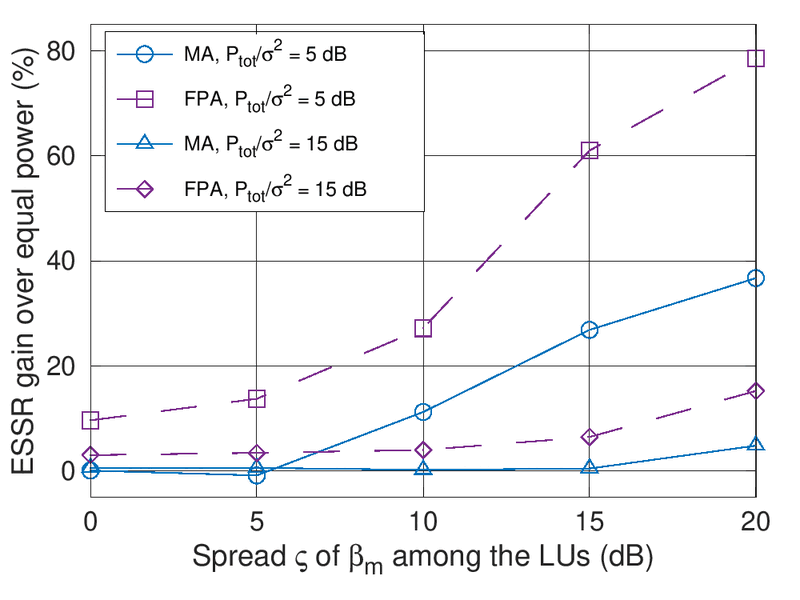
\includegraphics[width=\linewidth]{r1_fig8}\caption{Round 1 (invalid benchmark)}\end{subfigure}\hfill
\begin{subfigure}{0.46\textwidth}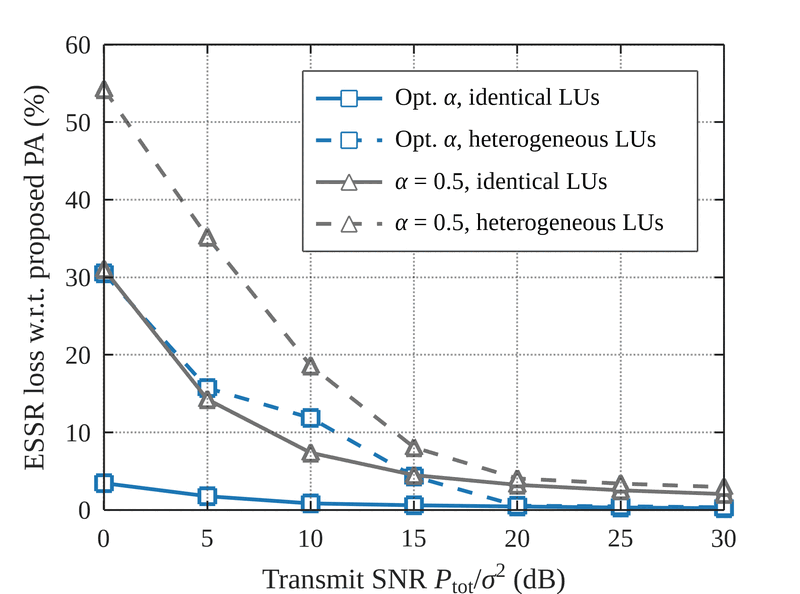
\includegraphics[width=\linewidth]{r2_fig8}\caption{Round 2}\end{subfigure}\\[4pt]
\begin{subfigure}{0.46\textwidth}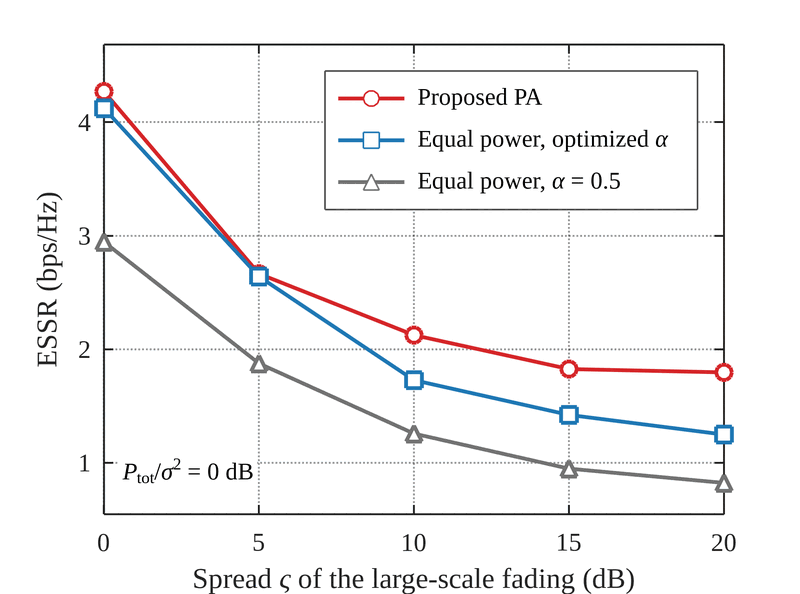
\includegraphics[width=\linewidth]{r3_fig8a}\caption{Round 3, 0~dB (old manuscript)}\end{subfigure}\hfill
\begin{subfigure}{0.46\textwidth}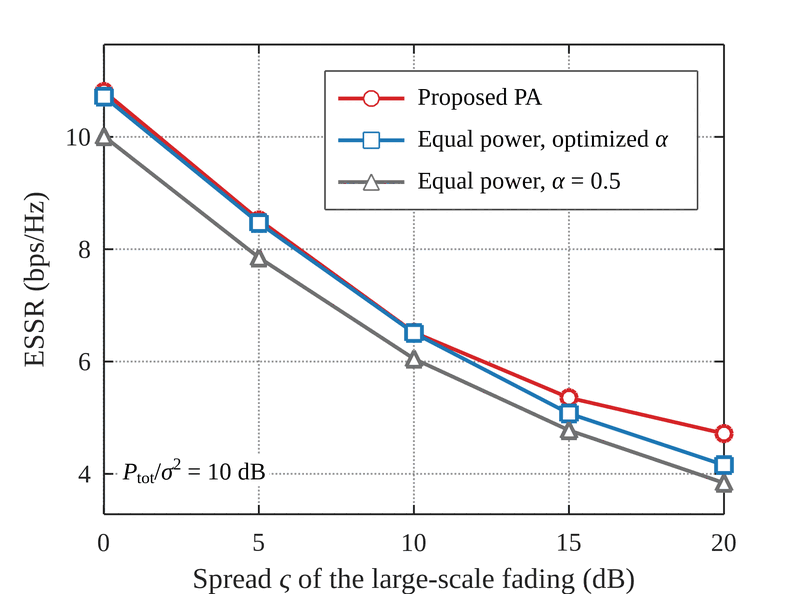
\includegraphics[width=\linewidth]{r3_fig8b}\caption{Round 3, 10~dB (old manuscript)}\end{subfigure}\\[4pt]
\begin{subfigure}{0.46\textwidth}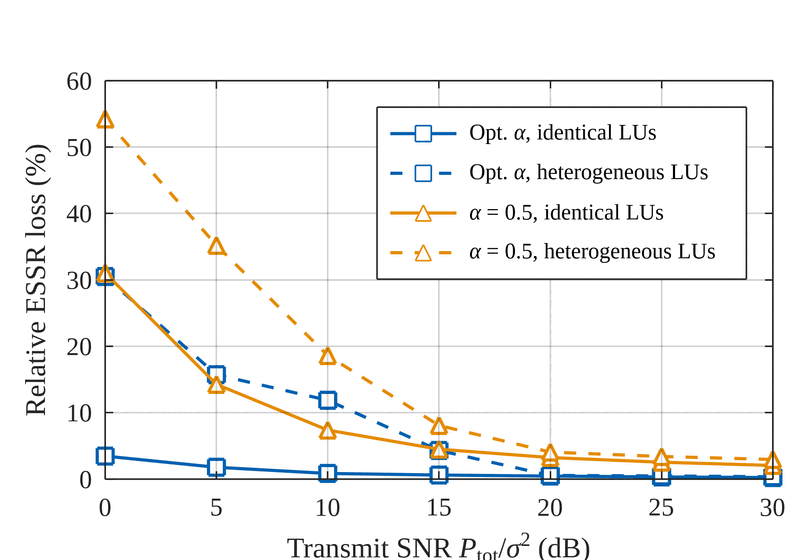
\includegraphics[width=\linewidth]{new_fig7_power_allocation}\caption{New Fig.~7 (round-2 design, new style)}\end{subfigure}
\caption{All versions of the power-allocation figure.}
\label{fig:cmp8}
\end{figure}

% =============================================================================
\section{Summary of changes}
% =============================================================================
\paragraph{Manuscript (\code{main.tex}, 13 pages).}
\begin{itemize}
\item Abstract (248 words) and contributions: AS claim qualified; robustness results mentioned.
\item Sections~I--IV: condensed as described in Section~\ref{sec:q1}; Table~I removed; Remark~2 inlined; the objective-value convergence statement made precise; references reordered by first citation.
\item Section~V rewritten for the new figure set: V-A one FPA (sparse FPA in one sentence), the w/o-AN design defined; V-B approximation gaps at the optimized designs; V-C single-panel convergence; V-D new paragraph on the AoD error of Eve; V-E region size with the region-wide AS, the angular offset, and the single LU in text; V-F new Fig.~7.
\item Figures: Fig.~3 (stacked axes), Fig.~4 (one panel), Fig.~5 (four schemes), Fig.~6 = old Fig.~7 (four schemes), Fig.~7 = restored round-2 power-allocation design. The old Fig.~6 was removed.
\end{itemize}

\paragraph{Code (\code{ma\_secrecy\_matlab}).}
\begin{itemize}
\item New: \code{design\_scenario.m} (statistical CSI at the BS, optional AoD error of Eve), \code{extra\_eve\_aod\_error.m}, \code{extra\_as\_region.m}, \code{style\_axes.m}, \code{axes\_note.m}, \code{print\_sweep.m}.
\item Changed: \code{evaluate\_schemes.m} (designs evaluated on the true scenario; scheme \code{'AS\_region'}), \code{as\_select.m} (optional candidates), \code{sweep\_schemes.m}, \code{main\_schemes.m} (four schemes), all plotting functions, \code{run\_all.m}, \code{replot\_all.m}, \code{default\_params.m} (\code{eveAoDErr} added, \code{fig8SNR} removed).
\item Renamed to match the new figure numbers: \code{fig7\_region.m}$\to$\code{fig6\_region.m}; \code{fig8\_power\_allocation.m}$\to$\code{extra\_pa\_spread.m} (the $\varsigma$ sweep); the new \code{fig7\_power\_allocation.m} reproduces the round-2 design; \code{fig6a\_angle.m}$\to$\code{extra\_angle\_offset.m}; \code{fig6b\_single\_user.m}$\to$\code{extra\_single\_user.m}; \code{print\_table2.m}$\to$\code{print\_table\_eve.m}. The results files were renamed accordingly, and the round-2 data were restored as \code{fig7\_pa\_identical.mat} and \code{fig7\_pa\_hetero.mat}.
\item Checks: \code{check\_implementation} passes (gradient error $1.3\times10^{-7}$, KKT, monotonicity); \code{run\_all} runs end to end in \code{QUICK} mode; the new code path reproduces the stored Fig.~5 values exactly; the readme (\code{readme.pdf}) was updated, including the new equation numbers.
\end{itemize}

\paragraph{For the authors to confirm.}
\begin{enumerate}
\item Run \code{replot\_all} in MATLAB once to obtain vector PDFs for the submission.
\item Decide whether the region-wide AS should become a curve in Fig.~6 (currently text only; see Section~\ref{sec:m4}).
\item Author information, funding, and the publication status of the arXiv references [14], [15].
\end{enumerate}

\end{document}
